\textbf{Agenda}

Pada chapter ini kita akan membahas beberapa topik tentang 
teknis polimorfisme, adapun topik yang akan dibahas
adalah

\minitoc

Secara teknis polimorfisme merupakan suatu konsep untuk merelasikan
diatara kelas-kelas C++ melalui overriding metode-metode virtual,
sehingga dengan demikian satu tipe kelas dapat konversikan menjadi kelas
lain. Aspek penting pertama dalam Pewarisan (\emph{Inheritance}) adalah
pengoganisasian kelas yang mengijinkan kelas lain berbagi program dan
data (\emph{code reuse}) sehingga progam tidak harus dibangun ulang dari
awal. Aspek penting kedua dari Pewarisan (\emph{Inheritance}) adalah
pengelompokan fitur-fitur kelas yang serupa kedalam sebuah kelas dasar
(\emph{base class}) dan kemudian membuat kelas lain dengan cara
menurunkan kelas tersebut sehingga bentuk utama/ pokok dari kelas-kelas
turunan menjadi serupa dengan kelas dasar sedemikian rupa sehingga
\texttt{pointer} atau referensi bertipe kelas dasar dapat menerima nilai
berbagai macam bentuk objek bertipe kelas turunannya (berubah tipe
kelas) dan dapat mengeksekusi fitur-fitur yang serupa tesebut. Inilah
yang disebut dengan polimorfisme.

Berbeda dengan tipe data standard (int, float, double, bool, dsb.) yang
jenisnya terbatas dan sudah pasti dikenal dalam pemrograman C++, kelas
adalah tipe data terstruktur yang bisa dibuat sendiri oleh programer,
sehingga tidak terbatas ada berapa macam kelas dalam C++. Namun di sisi
lain, dalam pemrograman kita pasti perlu untuk dapat berhubungan antara
kelas satu dengan yang lain, sehingga diperlukan suatu kerangka yang
dapat memberikan arahan mengenai bentuk dan fitur dari suatu kelas
sehingga dengan demikian ada suatu pointer atau referensi yang dapat
menerima berbagai macam bentuk yang dinamakan polimorfisme.

Mekanisme untuk dapat terjadi polimorfisme adalah pewarisan
(inheritance), oleh karena itu polimorfisme hanya bisa terjadi diantara
kelas-kelas yang mempunyai hubungan kekerabatan, tepatnya pointer atau
referensi bertipe kelas dasar hanya dapat menerima berbagai macam bentuk
objek yang bertipe kelas-kelas turunannya, sehingga pointer atau
referensi tersebut dapat mengeksekusi fitur-fitur yang serupa dengannya.
Contoh sederhana dari polimorfisme adalah seperti sudah dibahas pada bab
7 yaitu mengenai metode vitual pada percobaan Contoh 10.

Berikut ini akan dibahas secara lebih mendalam mengenai berbagai aspek
polimorfisme dari problem pada \texttt{single\ inheritance},
\texttt{multiple\ inheritance} hingga \texttt{abstract\ data\ type}.

\section{Problema Pewarisan Tunggal (Single Inheritance)}\label{problema-pewarisan-tunggal-single-inheritance}

Supaya terlihat sederhana, untuk menjelaskan masalah ini marilah kita
menggunakan ilustrasi mengenai kelas-kelas dengan perumpamaan kelas
binatang dan turunan-turunanya. Misalnya kelas Binatang mempunai hirarki
keturuan \textbf{Mamalia} dan \textbf{Burung}, kelas \texttt{Burung}
mempunyai member function \texttt{terbang()}, sedangkan kelas
\texttt{Mamalia} sudah diturunkan menjadi beberapa kelas diantaranya
\texttt{Kuda} dan \texttt{Anjing}. Kelas Kuda mempunyai member fucntion
\texttt{meringkik()} dan \texttt{melompat()}. Suatu saat terpikir untuk
membuat kelas \texttt{Kuda\_terbang} yang merupakan kombinasi antara
kelas \texttt{Burung} dan kelas \texttt{Kuda}, karena
\texttt{Kuda\_terbang} bisa \texttt{terbang()}, \texttt{meringkik()} dan
\texttt{melompat()}.

\begin{figure}[htbp]
\centering
\includegraphics[width=0.6\textwidth]{images/capture8-1.png}
\caption{Problema Pewarisan Tunggal (Single Inheritance}
\end{figure}

Dengan single inheritance hal ini tidak bisa dilakukan dengan mudah,
karena hanya bisa menurunkan dari salah satu kelas yang sudah ada, kita
bisa membuat \texttt{Kuda\_terbang} adalah turunan Burung yang bisa
\texttt{tebang()} tetapi akibatnya tidak bisa \texttt{meringkik()} dan
\texttt{melompat()}, sebaliknya jika dibuat sebagai turunan dari Kuda
akan bisa \texttt{meringkik()} dan \texttt{melompat()} tatapi tidak bisa
\texttt{terbang()}.

Untuk memaksakan hal ini bisa dilakukan dengan membuat metode
\texttt{terbang()} di dalam kelas \texttt{Kuda\_terbang} dan kelas ini
diturunkan dari kelas Kuda. Ini akan dapat dilakukan, akan tetapi harga
yang harus dibayar sekarang adalah kita mempunyai metode
\texttt{terbang()} dalam dua kelas yang berbeda (\texttt{Burung} dan
\texttt{Kuda\_terbang}), jika ada perubahan di salah satu metode
\texttt{terbang()}, maka harus selalu diingat untuk merubah yang
lainnya, ini sangat berisiko akan adanya ketidakkonsistenan program.

Belum lagi nanti akan timbul masalah \emph{polimorfisme} ketika akan
dibuat daftar objek Kuda atau daftar objek Burung, kalau
\texttt{Kuda\_terbang} dapat dimasukkan ke dalam dafatar Kuda maka ia
tidak akan bisa dimasukkan kedalam daftar Burung. Akibatnya akan timbul
ide untuk mengubah metode \texttt{melompat()} pada Kuda menjadi
\texttt{berpindah()} kemudian melakukan override dalam kelas
Kuda\_terbang yang melakukan pekerjaan \texttt{terbang()} dan pada
turunan Kuda lainnya melakukan override \texttt{berpindah()} yang
melakukan pekerjaan \texttt{melompat()}. Kemudian karena seharusnya
\texttt{Kuda\_terbang} tetap dapat melompat kita membatasi jika jarak
dekat melompat jika jarak jauh terbang seperti berikut:

\begin{lstlisting}[language=c++, numbers=none]
Kuda_terbang::berpindah(long jarak)
{
if (jarak > sangat_jauh)
terbang(jarak);
else
melompat(jarak);
}
\end{lstlisting}

Tapi ini menjadikan terbatas, bagaimana jika nanti ternyata
Kuda\_terbang bisa \texttt{melompat()} lebih jauh atau
\texttt{terbang()} lebih dekat? Ini akan menjadi masalah.

Solusi lainnya untuk membahas keterbatasan \emph{single inheritance} ini
adalah membuat metode \texttt{terbang()} pada kelas Kuda dan pada kelas
ini tidak melakukan \texttt{terbang()}, baru nanti kalau berupa objek
Kuda\_terbang, barulah \texttt{terbang()} yang sesungguhnya dikerjakan.
Marilah kita melakukan percobaan berikut ini.

\subsubsection*{Contoh  Meletakkan metode kelas turunan di kelas dasar.}

\begin{enumerate}

\item
  Buka Qt Creator dan buat project Qt Console Application baru dengan
  nama Contoh \ref{contoh-1}, kemudian tulis kode berikut.

\begin{lstlisting}[language=c++, caption= Meletakkan metode kelas turunan di kelas dasar, label=contoh-1]
#include <QtCore/QCoreApplication>
#include <iostream>
using namespace std;
class Kuda{
public:
void melompat(){ cout << "Lompat!" << endl;}
virtual void terbang(){cout <<"kuda tidak bisa terbang" << endl;}
};
class Kuda_terbang : public Kuda{
public:
void terbang() {cout << "terbang..." << endl;}
};
int main(int argc, char *argv[])
{
QCoreApplication a(argc, argv);
Kuda* kandang[5];
Kuda* kudanya;
int pilih;
for(int nomor=0; nomor<5; nomor++){
cout << "Pilih (0) Kuda atau (1) Kuda terbang : ";
cin >> pilih;
if(pilih==0)
kudanya = new Kuda();
else
kudanya = new Kuda_terbang();
kandang[nomor] = kudanya;
}
cout << endl;
for(int nomor=0; nomor<5; nomor++){
kandang[nomor]->terbang();
delete kandang[nomor];
}
return a.exec();
}
\end{lstlisting}
\item
  Kemudian jalankan kode diatas dengan menekan tombol Ctrl+R, outputnya
  adalah sebagai berikut.
\end{enumerate}

\begin{lcverbatim}
Pilih (0) Kuda atau (1) Kuda terbang : 0
Pilih (0) Kuda atau (1) Kuda terbang : 0
Pilih (0) Kuda atau (1) Kuda terbang : 1
Pilih (0) Kuda atau (1) Kuda terbang : 1
Pilih (0) Kuda atau (1) Kuda terbang : 0

kuda tidak bisa terbang
kuda tidak bisa terbang
terbang...
terbang...
kuda tidak bisa terbang
\end{lcverbatim}

\textbf{Analisa Program :}

\begin{itemize}
\item
  Pada program diatas ada dua kelas, yaitu Kuda sebagai kelas dasar dan
  \texttt{Kuda\_terbang} sebagai kelas turunan, Kuda mempunyai metode
  \texttt{terbang()} yang sebenarnya diada-adakan supaya bisa terjadi
  proses polimorfisme dengan baik, akibatnya metode \texttt{terbang()}
  ini tidak melakukan terbang yang sesungguhnya. Kelas
  \texttt{Kuda\_terbang} melakukan override terhadap metode virutal
  \texttt{terbang()}, pada metode ini melakukan terbang yang
  sesungguhnya.
\item
  Pada program utama disediakan program untuk menentukan 5 jenis kuda,
  yang ditampung dalam pointer kudanya. Pointer ini bisa berpolimorfisme
  kaena memenuhi syarat bahwa dia bertipe kelas dasar (Kuda) dan
  memanggil metode virutual terbang().
\item
  Pada percobaan eksekusi di atas dipilih 0, 0, 1, 1, 0 yang berarti
  array kandang berisi :

\begin{lstlisting}[language=c++, numbers=none]
Kandang[0] <-- berisi objek Kuda 
Kandang[1] <-- berisi objek Kuda 
Kandang[2] <-- berisi objek Kuda_terbang 
Kandang[3] <-- berisi objek Kuda_terbang 
Kandang[4] <-- berisi objek Kuda 
\end{lstlisting}

  Sehingga hasil keluaran berikutnya:

\begin{lstlisting}[language=c++, numbers=none]
kuda tidak bisa terbang 
kuda tidak bisa terbang 
terbang... 
terbang... 
kuda tidak bisa terbang
\end{lstlisting}
\item
  Dari percobaan ini tampak \emph{polimorfisme} bisa berhasil dengan
  baik. Namun seperti sudah dijelaskan di atas, harga yang harus dibayar
  adalah sekarang ada metode \texttt{terbang()} pada kelas
  \texttt{Kuda\_terbang} dan \texttt{Burung}, sehingga jika ada
  perubahan di salah satu metode \texttt{terbang()}, maka harus selalu
  diingat untuk merubah yang lainnya, ini sangat berisiko akan adanya
  ketidakkonsistenan program.
\end{itemize}
\begin{quotation}
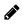
\includegraphics{images/pencil}	\textbf{Catatan:}
	
	Pada
	percobaan ini kelas telah disederhanakan untuk fokus pada pokok masalah
	yang hendak dijelaskan. Konstruktor, destruktor dan sebagainya
	dihilangkan supaya program tampak sederhana untuk membahas masalah
	\emph{single inheritance}. Tidak direkomendasikan untuk menulis program
	yang seperti ini.
\end{quotation}


\section{Peletakan ke atas (Pecolating
Upward)}\label{peletakan-ke-atas-pecolating-upward}

Meletakkan fungsi yang diperlukan pada kelas yang berada pada hierarki
di atasnya, seperti percobaan di atas, adalah solusi yang biasa
digunakan untuk keperluan polimorfisme dan juga dalam hal ini mengatasi
single inheritance dan berakibat menghasilkan banyak fungsi-fungsi
``yang diletakkan di atas'' (``Percolating up'') ke dalam kelas dasar.
Kemudian kelas dasar tersebut akan menjadi sangat berbahaya karena
menjadi global namespace untuk semua fungsi yang mungkin diperlukan
kelas turunan yang berpotensi merusak tatanan tipe kelas C++ dan
menciptakan kelas dasar yang berukuran besar dan tidak efisien.

Sebenarnya kejadian ini terjadi karena keinginan untuk menaruh
fungsionalitas bersama ke hirarki di atasnya tanpa mengubah antarmuka
(interface) dari tiap kelas. Artinya jika ada dua kelas yang memakai
kelas dasar yang sama (misalnya \texttt{Burung} dan \texttt{Kuda}
sama-sama bersal dari kelas dasar Binatang) dan keduanya sama-sama
mempunyai sebuah fungsi yang sama (misalnya Burung dan Kuda sama-sama
bisa makan), maka akan timbul ide untuk memindahkan fungsi tersebut ke
hirarki di atasnya dan membuat metode virtual pada kelas dasar.

\section{Konversi ke bawah (Casting
Down)}\label{konversi-ke-bawah-casting-down}

Alternatif lain untuk mengatasi single inheritance adalah tetap membuat
metode \texttt{terbang()} dalam kelas \texttt{Kuda\_terbang} dan metode
ini hanya dipanggil jika pointer menunjuk objek bertipe
\texttt{Kuda\_terbang}. Untuk keperluan ini diperlukan untuk dapat
mendeteksi objek tipe apa yang sedang ditunjuk oleh pointer yang dikenal
sebagai Runtime Type Identification (RTTI).
\begin{quotation}
	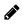
\includegraphics{images/pencil} \textbf{Catatan:}
	 
	 Hati-hati dalam menggunakan RTTI dalam program. Kebutuhan untuk memakai
	 RTTI bisa menjadi pertanda adanya desain hirarki pewarisan yang kurang
	 baik. Untuk itu sebaiknya gunakan metode virtual, template atau multiple
	 inheritance daripada memakai RTTI.
\end{quotation}


Pada percobaan Contoh 1 di atas, kita menunjuk baik Kuda maupun
\texttt{Kuda\_terbang}dengan array Kuda (kandang). Semuanya dimasukkan
sebagai Kuda. Dengan RTTI, kita akan memeriksa tiap-tiap elemen array
apakah objek yang ditunjuk berupa Kuda atau sebenarnya
\texttt{Kuda\_terbang}.

Pada percobaan ini kita tidak melakukan ``percolating upward'', yaitu
menuliskan metode \texttt{terbang()} ke dalam kelas Kuda melainkan
melakukan ``down casting'' untuk memanggil metode \texttt{terbang()}.
Untuk memanggil metode \texttt{terbang()} tersebut harus dipastikan
bahwa pointer sedang menunjuk objek bertipe Kuda\_terbang, bukan Kuda.
C++ mendukung ``down casting'' (RTTI) memakai operator
\texttt{dynamic\_cast}. Cara kerja \texttt{dynamic\_cast} adalah
demikian, jika kita memiliki pointer bertipe kelas dasar seperti Kuda
dan digunakan untuk menunjuk objek bertipe kelas turunan misalnya
\texttt{Kuda\_Terbang}, maka pointer tersebut bisa langsung dipergunakan
secara polimorfisme. Kemudian jika kita ingin mengambil objek
\texttt{Kuda\_terbang} yang sudah ditunjuk oleh pointer bertipe Kuda itu
dapat dilakukan dengan cara membuat pointer bertipe
\texttt{Kuda\_terbang} kemudian gunakan operator \texttt{dynamic\_cast}
untuk mengkonversikannya. Pada saat eksekusi (runtime), pointer dasar
akan diperiksa, jika sesuai maka pointer \texttt{Kuda\_terbang} bekerja
dengan baik, jika tidak sesuai maka sebenarnya bukan objek
\texttt{Kuda\_terbang} yang ditunjuk meliankan pointer kosong (null).
Lakukan percobaan berikut ini.

\subsubsection*{Contoh  Melakukan Down Casting.}

\begin{enumerate}

\item
  Buka Qt Creator dan buat project Qt Console Application baru dengan
  nama Contoh \ref{contoh-2}, kemudian tulis kode berikut.

\begin{lstlisting}[language=c++, caption= Melakukan Down Casting, label=contoh-2]
#include <QtCore/QCoreApplication>
#include <iostream>
using namespace std;
class Kuda{
public:
virtual void melompat(){ cout << "Lompat!" << endl;}
};
class Kuda_terbang : public Kuda{
public:
virtual void terbang() {cout << "terbang..." << endl;}
};
int main(int argc, char *argv[])
{
QCoreApplication a(argc, argv);
Kuda* kandang[5];
Kuda* kudanya;
int pilih;
for(int nomor=0; nomor<5; nomor++){
cout << "Pilih (0) Kuda atau (1) Kuda terbang : ";
cin >> pilih;
if(pilih==0)
kudanya = new Kuda();
else
kudanya = new Kuda_terbang();
kandang[nomor] = kudanya;
}
cout << endl;
for(int nomor=0; nomor<5; nomor++){
Kuda_terbang *pKterb = dynamic_cast<Kuda_terbang*> (kandang[nomor]);
if (pKterb != NULL)
pKterb->terbang();
else
cout << "Kuda biasa " << endl;
delete kandang[nomor];
}
return a.exec();
}
\end{lstlisting}
\item
  Kemudian jalankan kode diatas dengan menekan tombol Ctrl+R, outputnya
  adalah sebagai berikut.
\end{enumerate}

\begin{lcverbatim}
Pilih (0) Kuda atau (1) Kuda terbang : 1
Pilih (0) Kuda atau (1) Kuda terbang : 0
Pilih (0) Kuda atau (1) Kuda terbang : 1
Pilih (0) Kuda atau (1) Kuda terbang : 0
Pilih (0) Kuda atau (1) Kuda terbang : 1

terbang...
Kuda biasa
terbang...
Kuda biasa
\end{lcverbatim}

\textbf{Analisa Program :}

\begin{itemize}

\item
  Jalan keluar single inheritance ini berjalan dengan baik, namun tidak
  direkomendasikan untuk memakai cara ini. Hasilnya hanya berupa
  tambal-sulam saja, sebenarnya metode \texttt{terbang()} tidak ada di
  kelas Kuda dan tidak dipanggil dari sana. Ketika dipanggil dengan
  poiter \texttt{Kuda\_terbang} dilakukan casting secara eksplisit, maka
  harus dipastikan bahwa pointer pKterb benar-bena berisi objek bertipe
  \texttt{Kuda\_terbang} sebelum memanggil metode \texttt{terbang()}.
\item
  Pemakain down casting semacam ini merupakan pertanda bahwa desain yang
  dibuat kurang baik, program semacam ini merusak fungsi \emph{virtual
  polimorfisme} karena ini dilakukan \texttt{casting} objek menjadi tipe
  yang sesungguhnya (bukan polimorfisme).
\end{itemize}

\section{Menambahkan ke Dua Daftar}\label{menambahkan-ke-dua-daftar}

Masalah lain yang dihadapi oleh karena memakai solusi di atas adalah
bahwa kita telah mendeklarasikan \texttt{Kuda\_terbang} bertipe Kuda,
sehingga kita tidak bisa menambahkan objek \texttt{Kuda\_terbang} ke
dalam daftar objek Burung. Dalam hal ini bisa saja kita melakukan
pemindahan metode \texttt{terbang()} ke hirarki atasnya yaitu kedalam
kelas Kuda atau melakukan down casting pada pointer, tetapi tetap saja
kita tidak mendapatkan fungsionalitasnya secara penuh.

Satu solusi terakhir untuk mengatasi masalah single inheritance ini
adalah memindahkean semua fungsi \texttt{terbang()},
\texttt{meringkik()} dan \texttt{melompat()} ke kelas dasar dari Burang
dan Kuda, yaitu kelas Binatang. Dengan demikian kita bisa mendaftar
objek-objek Burung, Kuda maupun objek-objek \texttt{Kuda\_terbang} dalam
satu kesatuan daftar Binatang. Namun akibatnya kelas dasar mempunyai
semua karakteristik kelas turunannya sehingga ukuran kelas dasar menjadi
sangat besar dan ini tidak diinginkan.

\section{Pewarisan Ganda (Multiple
Inheritance)}\label{pewarisan-ganda-multiple-inheritance}

Dengan C++ dimungkinkan untuk menurunkan kelas baru yang berasal dari
lebih dari satu kelas dasar, yang dinamakan pewaisan ganda (multiple
inheritance). Penurunan lebih dari satu kelas dasar dilakukan dengan
cara menuliskan kelas dasar berikutnya dipisahkan dengan tanda koma (,)
seperti berikut:

\begin{lstlisting}[language=c++, numbers=none]
class KelasTurunan : public KelasDasar1, public KelasDasar2{}
\end{lstlisting}

Percobaan berikut ini memberikan ilustrasi cara deklarasi kelas
\texttt{Kuda\_terbang} yang mewarisi kelas dasar Kuda dan Burung,
kemudian program menambahkan objek Kuda\_terbang ini di kedua jenis
daftar objek tersebut.

\subsubsection*{Contoh Multiple Inheritance.}

\begin{enumerate}

\item
  Buka Qt Creator dan buat project Qt Console Application baru dengan
  nama Contoh \ref{contoh-3}, kemudian tulis kode berikut.

\begin{lstlisting}[language=c++, caption=Multiple Inheritance, label=contoh-3]
#include <QtCore/QCoreApplication>
#include <iostream>
using namespace std;
class Kuda{
public:
Kuda() {cout << "Konstruktor Kuda ... ";}
virtual ~Kuda() {cout << "Destruktor Kuda ... \n";}
virtual void meringkik() const {cout << " Kikikikikkkk...";}
};
class Burung{
public:
Burung() { cout << "Konstruktor Burung ... "; }
virtual ~Burung() { cout << "Destruktor Burung ... "; }
virtual void berkicau() const { cout << " Cicit cuit... "; }
virtual void terbang() const { cout << " Terbang ... "; }
};
class Kuda_terbang : public Kuda, public Burung{
public:
void berkicau() const { meringkik(); }
Kuda_terbang() { cout << "Konstruktor Kuda_terbang ... "; }
~Kuda_terbang() { cout << "Destruktor Kuda_terbang ... "; }
};
int main(int argc, char *argv[])
{
QCoreApplication a(argc, argv);
Kuda* daftar_kuda[2]; //<-- kumpulan Kuda
Burung* daftar_burung[2]; //<-- kumpulan Burung
cout << "Menciptakan objek Kuda:" << endl;
daftar_kuda[0] = new Kuda(); //<-- objek Kuda
cout << "\nMenciptakan objek Kuda_terbang:" << endl;
daftar_kuda[1] = new Kuda_terbang(); //<-- objek Kuda_terbang
cout << "\nMenciptakan objek Burung:" << endl;
daftar_burung[0] = new Burung(); //<-- objek Burung
cout << "\nMenciptakan objek Kuda_terbang:" << endl;
daftar_burung[1] = new Kuda_terbang();//<-- objek Kuda_terbang
cout << "\n\nTampilkan daftar_kuda :" << endl;
daftar_kuda[0]->meringkik(); //<-- berisi objek Kuda
cout << "\nHapus Kuda : ";
delete daftar_kuda[0];
daftar_kuda[1]->meringkik(); //<-- berisi objek Kuda_terbang
cout << "\nHapus Kuda_terbang : ";
delete daftar_kuda[1];
cout << "\nTampilkan daftar_burung :" << endl;
daftar_burung[0]->berkicau(); //<-- berisi objek Burung
daftar_burung[0]->terbang(); //<-- berisi objek Burung
cout << "\nHapus Burung : " ;
delete daftar_burung[0];
cout << endl;
daftar_burung[1]->berkicau(); //<-- berisi objek Kuda_terbang
daftar_burung[1]->terbang(); //<-- berisi objek Kuda_terbang
cout << "\nHapus Kuda_terbang : ";
delete daftar_burung[1];
return a.exec();
}
\end{lstlisting}
\item
  Kemudian jalankan kode diatas dengan menekan tombol Ctrl+R, outputnya
  adalah sebagai berikut.
\end{enumerate}

\begin{figure}[htbp]
\centering
\includegraphics[width=0.8\textwidth]{images/capture9-1.png}

\end{figure}

\textbf{Analisa Program :}

\begin{itemize}
\item
  Pada kelas \texttt{Kuda\_terbang} tampak penggunaan multiple
  inheritance, yaitu pada deklarasikelas \texttt{Kuda\_terbang} yang
  merupakan keturunan dari Kuda dan Burung :

\begin{lstlisting}[language=c++, numbers=none]
class Kuda_terbang : public Kuda, public Burung
\end{lstlisting}
\item
  Kemudian kelas ini melakukan override terhadap metode
  \texttt{berkicau()}, metode \texttt{berkicau()} pada
  \texttt{Kuda\_terbang} ini mengerjakan pemanggilan metode
  \texttt{meringkik()}, yaitu metode warisan dari kelas Kuda:

\begin{lstlisting}[language=c++, numbers=none]
void berkicau() const { meringkik(); }
\end{lstlisting}
\item
  Tampak pada percobaan Contoh 3 ini ketika diciptakan objek bertipe
  Kuda maka yang bekerja adalah konstruktor \texttt{Kuda}, demikian juga
  ketika diciptakan objek \texttt{Burung} yang bekerja adalah
  konstruktor \texttt{Burung}, namun ketika diciptakan
  \texttt{Kuda\_terbang} yang bekerja tiga konstruktor sekaligus, yaitu
  : konstruktor \texttt{Kuda}, konstruktor \texttt{Burung} dan
  konstruktor \texttt{Kuda\_terbang}. Ini mempelihatkan bahwa kelas
  \texttt{Kuda\_terbang} merupakan turunan dari kelas Kuda sekaligus
  turunan kelas \texttt{Burung}. Dengan kata lain objek
  \texttt{Kuda\_terbang} adalah objek yang di dalamnya terkandung bagian
  objek Kuda dan bagian objek Burung.
\item
  Kebalikannya saat dihapus, destruktor yang dijalankan : destruktor
  \texttt{Kuda\_terbang}, destruktor Burung baru kemudian destruktor
  Kuda. Ini adalah akibat adanya destruktor yang selalu virtual.
\item
  Pada saat ditampilkan \texttt{daftar\_kuda}, tampak pada program
  sebenarnya yang pertama berisi objek Kuda sedangkan yang kedua berisi
  objek \texttt{Kuda\_terbang} :

\begin{lstlisting}[language=c++, numbers=none]
daftar_kuda[0] = new Kuda(); //<-- objek Kuda
daftar_kuda[1] = new Kuda_terbang(); //<-- objek Kuda_terbang
\end{lstlisting}
\item
  Demikian juga pada daftar\_burung, yang pertama berisi objek Burung
  sedangkan yang kedua berisi Kuda\_terbang :

\begin{lstlisting}[language=c++, numbers=none]
daftar_burung[0] = new Burung(); //<-- objek Burung
daftar_burung[1] = new Kuda_terbang();//<-- objek Kuda_terbang
\end{lstlisting}
\item
  Ini menunjukkan bahwa baik \texttt{daftar\_kuda{[}{]}} maupun
  \texttt{daftar\_burung{[}{]}} dapat berpolimorfisme dengan sempurna
  berkat adanya multiple inheritance.
\item
  Pada waktu \texttt{daftar\_burung} berisi objek Kuda\_terbang, ketika
  dipanggil metode berkicau berikut :

\begin{lstlisting}[language=c++, numbers=none]
daftar_burung[1]->berkicau(); //<-- berisi objek Kuda_terbang
\end{lstlisting}
\item
  Maka yang menanggapi adalah metode hasil override di dalam kelas
  \texttt{Kuda\_terbang} yaitu pemanggilan metode \texttt{meringkik()},
  sehingga keluarannya adalah :

\begin{lstlisting}[language=c++, numbers=none]
" Kikikikikkkk..."
\end{lstlisting}
\end{itemize}

\section{Komponen Objek Multi
Inheritance}\label{komponen-objek-multi-inheritance}

Ketika objek Kuda\_terbang diciptakan di memori, kedua kelas dasarnya
juga tercipta sebagai bagian pembentuk objek tersebut. Gambar di bawah
ini menggambarkan sebuah objek bertipe Kuda\_terbang termasuk
fitur-fitur baru yang ditambahkan pada kelas Kuda\_terbang maupun
fitur-fitur warisan kelaskelas dasarnya.

\begin{figure}[htbp]
\centering
\includegraphics{images/capture9-2.png}
\caption{}
\end{figure}

Ada beberapa hal yang perlu diperhatikan pada objek yang merupakan
turunan dari beberapa kelas dasar. Sebagai contoh misalnya, apa yang
terjadi jika kedua kelas dasar tersebut memiliki metode virtual atau
data yang sama? Bagaimana cara menginisialisasi konstruktor kelas
dasarnya? Bagaimana jika kedua kelas dasar yang diturunkan merupakan
keturunan dari suatu kelas dasar yang sama? Berikut ini akan kita
bicarakan mengenai isu-isu tersebut.

\section{Konstruktor Kelas Banyak Turunan (Multiple
Inheritance)}\label{konstruktor-kelas-banyak-turunan-multiple-inheritance}

Seperti pada umumnya, kelas turunan pasti memanggil konstruktor kelas
dasarnya, demikian juga konstruktor kelas banyak turunan (multiple
inheritance) juga harus memanggil konstruktor-kontruktor kelas dasarnya.
Jika bentuk konstruktor default (konstruktor yang diciptakan secara
otomatis oleh kompiler jika kelas turunan tidak menuliskan konstruktor
secara eksplisit) pada single inheritance yaitu:

\begin{lstlisting}[language=c++, numbers=none]
KelasTurunan():KelasDasar(){} //<-- Konstruktor default kelas Turunan tunggal
\end{lstlisting}

Maka konstruktor default kelas banyak turunan (mutiple inheritance)
adalah :

\begin{lstlisting}[language=c++, numbers=none]
KelasTurunan():KelasDasar1(),KelasDasar2(){}
\end{lstlisting}

Jadi pada waktu membuat kelas banyak turunan, khususnya jika kelas
dasarnya tidak mempunyai konstruktor tanpa parameter, maka konstruktor
kelas turunan tersebut harus memanggil salah satu dari konstruktor
kelas-kelas dasarnya, karena kalau tidak kompiler akan memanggil
konstruktor default kelas dasar yang sebenarnya tidak ada sehingga
menimbulkan kesalahan kompilasi.

Supaya bisa fokus pada pokok permasalahan, yaitu konstruktor, percobaan
berikut ini menghilangkan berbagai macam anggota yang lain supaya
terlihat sederhana dan mudah dipahami.

\subsubsection*{Contoh  Konstruktor Kelas Multiple Inheritance.}

Buka Qt Creator dan buat project Qt Console Application baru dengan nama
Contoh \ref{contoh-4}, kemudian tulis kode berikut.

\begin{lstlisting}[language=c++, caption=Konstruktor Kelas Multiple Inheritance, label=contoh-4]
#include <QtCore/QCoreApplication>
#include <iostream>
using namespace std;
class Kuda{
public:
Kuda(string nama){
cout << "Konstruktor Kuda, nama = " << nama << endl;
}
};
class Burung{
public:
Burung(string warna){
cout << "Konstruktor Burung, warna = " << warna << endl;
}
};
class Kuda_terbang : public Kuda, public Burung{
public:
Kuda_terbang():Kuda("Gondrong"),Burung("Merah"){
cout << "Konstuktor Kuda_terbang";
}
};
int main(int argc, char *argv[])
{
QCoreApplication a(argc, argv);
Kuda_terbang* gondrong = new Kuda_terbang();
return a.exec();
}
\end{lstlisting}

Kemudian jalankan kode diatas dengan menekan tombol Ctrl+R, outputnya
adalah sebagai berikut.

\begin{lcverbatim}
Konstruktor Kuda, nama = Gondrong
Konstruktor Burung, warna = Merah
\end{lcverbatim}

\textbf{Analisa Program :}

\begin{itemize}
\item
  Kelas Kuda hanya mempunyai \texttt{sebuah} konstruktor dengan sebuah
  parameter bertipe \texttt{string}, demikian juga kelas \texttt{Burung}
  hanya mempunyai sebuah konstruktor dengan \texttt{sebuah} parameter
  bertipe \texttt{string}.
\item
  Pada kelas \texttt{Kuda\_terbang} tampak penggunaan multiple
  inheritance, yaitu pada deklarasi kelas \texttt{Kuda\_terbang} yang
  merupakan keturunan dari Kuda dan Burung :

\begin{lstlisting}[language=c++, numbers=none]
class Kuda_terbang : public Kuda, public Burung
\end{lstlisting}
\item
  Oleh karena itu konstruktor kelas \texttt{Kuda\_terbang} ini harus
  memanggil secara eksplisit konstruktor-konstruktor kelas dasarnya
  seperti berikut:

\begin{lstlisting}[language=c++, numbers=none]
Kuda_terbang():Kuda("Gondrong"),Burung("Merah")
\end{lstlisting}
\item
  Tampak pada hasil output, instansiasi kelas Kuda\_terbang menjalankan
  konstruktor Kuda dengan satu parameter dan konstruktor Burung dengan
  satu parameter, baru kemudian menjalankan konstruktornya sendiri.
\end{itemize}

\section{Problem Ambiguitas}\label{problem-ambiguitas}

Pada kelas multi inheitance yang beberapa kelas dasarnya mempunyai
metode virtual yang sama akan menimbulkan masalah ketika objek kelas
turunan akan memanggil metode tersebut, sebab kelas tersebut mendapatkan
warisan dari keduanya, sehingga ketika metode tersebut dipanggil akan
menimbulkan masalah ambiguitas bagi kompiler.

Sebagai contoh misalnya kelas Kuda dan kelas Burung sama-sama mempunyai
metode \texttt{virutal\ makan()}dam jika kita memanggil metode dari
objek Kuda\_terbang yang merupakan multi inheritance dari kedua kelas
tersebut di atas.

\begin{lstlisting}[language=c++, numbers=none]
pKterbang->makan();
\end{lstlisting}

Maka kompile akan menampilkan pesan kesalahan :

\begin{lstlisting}[language=c++, numbers=none]
Member is ambiguous: 'Kuda::makan; and 'Burung::makan'
\end{lstlisting}

Untuk memecahkan masalah ini dengan pemanggilan secara eksplisit bisa
dilakukan dengan cara menyebutkan nama kelas dasar pemilik metode
virtual yang akan dieksekusi, misalnya:

\begin{lstlisting}[language=c++, numbers=none]
pKterbang->Kuda::makan();
\end{lstlisting}

Kapan saja kita ingin mengeksekusi fungsi anggota atau variabel anggota
kelas mana yang akan diakses, kita dapat melakukan dengan cara tersebut
di atas. Jika kelas Kuda\_terbang akan melakukan overriding fungsi
tersebut, maka pemanggilan tersebut bisa dilakukan di dalam fungsi
anggota Kuda\_terbang:

\begin{lstlisting}[language=c++, numbers=none]
virtual void makan() const { Kuda::makan() }
\end{lstlisting}

Dengan cara ini kita bisa menyembunyikan masalah ambiguitas ini dari
pemakai kelas Kuda\_terbang dengan cara mengenkapsulasi di dalam kelas
Kuda\_terbang mengenai kelas dasar mana yang diambil warisan fungsi
makan()-nya. Namun pemakai tetap saja bebas untuk dapat memanggil waisan
lainnya dengan menulis :

\begin{lstlisting}[language=c++, numbers=none]
pKterbang->Burung::makan();
\end{lstlisting}

\section{Penurunan dari Kelas Dasar
Bersama}\label{penurunan-dari-kelas-dasar-bersama}

Jika dua kelas dasar yang dijadikan multiple inheritance merupakan
turunan dari kelas dasar yang sama, maka ketika diciptakan objek dari
kelas turunan akan bisa terbentuk objek dengan 2 kemungkinan, yaitu:

\begin{enumerate}


\item
  Tercipta 2 objek kelas dasar (\textbf{Common Base Class})
\item
  Tercipta 1 Objek kelas dasar (\textbf{Diamond Inheritance})
\end{enumerate}

Sebagai ilustrasi seperti contoh sebelumnya, \texttt{Kuda} dan
\texttt{Burung} merupakan turunan dari sebuah kelas dasar yang sama
yaitu kelas \texttt{Binatang}, sedangkan \texttt{Kuda\_terbang}
merupakan hasil \emph{multiple inheritance} dari kelas \texttt{Kuda} dan
\texttt{Burung}. Pada saat \emph{instansiasi} kelas
\texttt{Kuda\_terbang} terdapat 2 kemungkinan bentuk kelas yang terjadi:

\begin{figure}[htbp]
\centering
\includegraphics[width=0.8\textwidth]{images/capture9-3.png}
\caption{Penurunan dari class dasar yang sama}
\end{figure}

\textbf{Common base class} adalah penurunan seperti biasa yang terjadi,
yaitu ketika kelas paling bawah (\texttt{Kuda\_terbang}) melakukan
instansiasi, secara otomatis kelas-kelas dasarnya (Kuda dan Burung) juga
terbentuk, dan ketika kedua kelas dasar tersebut terbentuk
(\texttt{Kuda} dan \texttt{Burung}), masing-masing memanggil secara
terpisah kostruktor kelas dasar paling atas (Binatang), sehingga
terbentuklah objek kelas dasar paling atas untuk masing-masing
(sendiri-sendiri). Sedangkan Diamon inheritance terjadi ketika dilakukan
penurunan secara virtual, yaitu konstruktor kelas turunan paling bawah
(\texttt{Kuda\_terbang}) memanggil secara langsung konstruktor kelas
dasar paling atas (Binatang), sehingga pemanggilan oleh kedua kelas
dasarnya (\texttt{Kuda} dan \texttt{Burung}) terhadap konstruktor kelas
dasar paling atas (\texttt{Binatang}) diabaikan. Hal ini bisa terjadi
jika penurunan dilakukan secara virtual yang akan dibahas nanti.

Untuk penurunan pada umumnya (Common base class) ada kemungkinan kelas
Kuda maupun Burung masing-masing sudah melakukan overriding terhadap
metode milik kelas dasarnya (Binatang). Sebagai contoh misalnya kelas
Binatang mempunyai member variabel umur dan member function getUmur().
Jika kelas turunan paling bawah (Kuda\_terbang) memanggil metode
getUmur() tersebut, makan akan timbul ambiguitas lagi, yaitu metode yang
dipanggil merupakan getUmur() Kuda atau getUmur() Burung? Pemecahan
problem ini sama dengan pada kelas multi inheitance yang yang kedua
kelas dasarnya mempunyai metode virtual yang sama, yaitu bisa dilakukan
dengan cara melakukan override terhadap metode \texttt{getUmur()} kemudian di
dalamnya memilih metode yang akan merespon, misalnya dipilih \texttt{getUmur()}
dari Kuda seperti berikut:

\begin{lstlisting}[language=c++, numbers=none]
virtual int getUmur() const { return Kuda::getUmur() }
\end{lstlisting}

Agar lebih jelas, lakukan pecobaan berikut ini.

\subsubsection*{Contoh  Penurunan pada umumnya (Common Base Class).}

Buka Qt Creator dan buat project Qt Console Application baru dengan nama
Contoh \ref{contoh-5}, kemudian tulis kode berikut.

\begin{lstlisting}[language=c++, caption= Penurunan pada umumnya (Common Base Class), label=contoh-5]
#include <QtCore/QCoreApplication>
#include <iostream>
using namespace std;
class Binatang{
public:
Binatang(int umur=5):umur(5){cout << "Konstruktor Binatang\n";}
~Binatang(){cout << "Destruktor Binatang\n";}
protected:
int umur;
public:
virtual int const getUmur(){
cout << "dari Binatang...";
return umur;
}
};
class Kuda : public Binatang{
public:
Kuda(){cout << "Konstruktor Kuda\n";}
~Kuda(){cout << "Destruktor Kuda\n";}
virtual int const getUmur(){
cout << "dari Kuda...";
return umur;
}
                                        
};
class Burung : public Binatang{
public:
Burung(){cout << "Konstruktor Burung\n";}
~Burung(){cout << "Destruktor Burung\n";}
virtual int const getUmur(){
cout << "dari Burung...";
return umur;
}
};
class Kuda_terbang : public Kuda, public Burung{
public:
Kuda_terbang(){cout << "Konstruktor Kuda_terbang\n";}
~Kuda_terbang(){cout << "Destruktor Kuda_terbang\n";}
virtual int const getUmur(){
cout << "dari Kuda_terbang...";
return Kuda::getUmur();
}
};
int main(int argc, char *argv[])
{
QCoreApplication a(argc, argv);
Kuda_terbang* gondrong = new Kuda_terbang();
cout << "Umur : " << gondrong->getUmur() << endl;
delete gondrong;
return a.exec();
}
\end{lstlisting}

Kemudian jalankan kode diatas dengan menekan tombol Ctrl+R, outputnya
adalah sebagai berikut.

A\textgreater{} \{linenos=off\} A\textgreater{} Konstruktor Binatang
A\textgreater{} Konstruktor Kuda A\textgreater{} Konstruktor Binatang
A\textgreater{} Konstruktor Burung A\textgreater{} Konstruktor
Kuda\_terbang A\textgreater{} dari Kuda\_terbang\ldots{}dari
Kuda\ldots{}Umur : 5

\textbf{Analisa Program :}

\begin{itemize}
\item
  Pada program Utama hanya menciptakan objek bertipe
  \texttt{Kuda\_terbang}. Tampak pada hasil keluaran, dilihat dari
  konstruktornya maka bisa disimpulkan bahwa terbentuk objek
  \texttt{Binatang}, objek \texttt{Kuda}, objek \texttt{Binatang}, objek
  \texttt{Burung} baru kemudian objek \texttt{Kuda\_terbang}. Ini
  menunjukkan bahwa ada 2 objek Binatang yang masing-masing merupakan
  bagian \texttt{Kuda} dan \texttt{Burung}.
\item
  Oleh karena \texttt{Kuda\_terbang} adalah turunan dari \texttt{Kuda}
  dan \texttt{Burung}, maka jika ia memanggil metode \texttt{getUmur()}
  yang merupakan warisan dari mereka, akan terjadi ambiguitas, oleh
  karena itu pada kelas \texttt{Kuda\_terbang} dilakukan overriding
  seperti berikut :

\begin{lstlisting}[language=c++, numbers=none]
virtual int const getUmur(){
cout << "dari Kuda_terbang...";
return Kuda::getUmur();
}
\end{lstlisting}
\item
  Tampak pada hasil pemanggilan metode tersebut pada kelas
  Kuda\_terbang: dari Kuda\_terbang\ldots{}dari Kuda\ldots{}Umur : 5 Ini
  menunjukkan bahwa metode yang dipanggil adalah metode hasil override
  pada kelas \texttt{Kuda\_tebang} yang di dalamnya sudah mengatasi
  problem ambiguitas dengan memastikan yang dipanggil adalah
  \texttt{getUmur()} dari kelas Kuda (yaitu : \texttt{Kuda::getUmur()}).
\item
  Sekali lagi pada saat objek dihapus (delete), destruktor yang
  dijalankan adalah untuk objek \texttt{Kuda\_terbang}, \texttt{Burung},
  \texttt{Binatang}, \texttt{Kuda} dan Binatang ini menunjukkan bahwa
  ada 2 objek Binatang tadi.
\end{itemize}

\section{Penurunan Virtual (Virtual
Inheritance)}\label{penurunan-virtual-virtual-inheritance}

Berbeda dengan penurunan biasa (\emph{Common Base Class}), penurunan
virtual pada kedua kelas dasar (Kuda dan Burung) menyebabkan kelas
turunan multi inheritance Kuda\_terbang dapat langsung memanggil
konstruktor kelas dasar paling atas (Binatang), sehingga terbentuklah
objek dengan bentuk Diamond Inheritance seperti gambar tadi. Supaya
lebih jelas, lakukan pecobaan berikut ini.

\subsubsection*{Contoh  Penurunan pada umumnya (Common Base Class).}

\begin{enumerate}

\item
  Buka Qt Creator dan buat project Qt Console Application baru dengan
  nama Contoh \ref{contoh-6}, kemudian tulis kode berikut.

\begin{lstlisting}[language=c++, caption= Penurunan pada umumnya (Common Base Class), label=contoh-6]
#include <QtCore/QCoreApplication>
#include <iostream>
using namespace std;
class Binatang{
public:
Binatang(int umur=5):umur(5){cout << "Konstruktor Binatang\n";}
~Binatang(){cout << "Destruktor Binatang\n";}
protected:
int umur;
public:
virtual int const getUmur(){
cout << "dari Binatang...";
return umur;
}
};
class Kuda : virtual public Binatang{
public:
Kuda(){cout << "Konstruktor Kuda\n";}
~Kuda(){cout << "Destruktor Kuda\n";}
};
class Burung : virtual public Binatang{
public:
Burung(){cout << "Konstruktor Burung\n";}
~Burung(){cout << "Destruktor Burung\n";}
};
class Kuda_terbang : public Kuda, public Burung{
public:
Kuda_terbang():Kuda(),Burung(),Binatang(){
cout << "Konstruktor Kuda_terbang\n";}
~Kuda_terbang(){cout << "Destruktor Kuda_terbang\n";}
};
int main(int argc, char *argv[])
{
QCoreApplication a(argc, argv);
Kuda_terbang* gondrong = new Kuda_terbang();
cout << "Umur : " << gondrong->getUmur() << endl;
delete gondrong;
return a.exec();
}
\end{lstlisting}
\item
  Kemudian jalankan kode diatas dengan menekan tombol Ctrl+R, outputnya
  adalah sebagai berikut.
\end{enumerate}
\begin{lcverbatim}
Konstruktor Binatang
Konstruktor Kuda 
Konstruktor Burung
Konstruktor Kuda_terbang dari
BinatangUmur : 5
\end{lcverbatim}


\textbf{Analisa Program :}

\begin{itemize}
\item
  Pada program Utama, sama seperti percobaan Contoh 5, hanya menciptakan
  objek bertipe Kuda\_terbang. Tampak pada hasil keluaran, dilihat dari
  konstruktornya maka bisa disimpulkan bahwa terbentuk objek Binatang,
  objek Kuda, objek Binatang, objek Burung baru kemudian objek
  Kuda\_terbang. Ini menunjukkan bahwa ada 2 hanya 1 objek Binatang yang
  masing-masing merupakan bagian Kuda, dan Burung dan Kuda\_terbang.
\item
  Walaupun Kuda\_terbang adalah turunan dari Kuda dan Burung, namun saat
  instansiasi kelas Kuda\_terbang memanggil langsung konstruktor
  Binatang seperti berikut:

\begin{lstlisting}[language=c++, numbers=none]
Kuda_terbang():Kuda(),Burung(),Binatang()
\end{lstlisting}
\end{itemize}

Memang kelas \texttt{Kuda\_terbang} bukan keturunan langsung kelas
Binatang, namun hal ini bisa dimungkinkan karena kelas dasar dari
\texttt{Kuda\_terbang}, yaitu Kuda dan Binatang melakukan penurunan
secara virutal :

\begin{lstlisting}[language=c++, numbers=none]
class Kuda : virtual public Binatang{}
class Burung : virtual public Binatang{}
\end{lstlisting}

sehingga dimungkinkan konstruktor \texttt{Kuda\_terbang()} memanggil
langsung konstruktor \texttt{Binatang()}. Konsekuensinya maka jika ia
memanggil metode \texttt{getUmur()} yang merupakan warisan dari
\texttt{Binatang}, metode-metode warisan yang ada pada \texttt{Kuda} dan
\texttt{Burung} akan diabaikan (kecuali mereka melakukan override) dan
di-``By pass'' langsung ke kelas Binatang. Oleh karena itu pada kelas
Kuda\_terbang tidak lagi terjadi ambigu seperti tadi. - Tampak pada
hasil pemanggilan metode \texttt{getUmur()} tersebut pada kelas
Kuda\_terbang: dari Binatang\ldots{}Umur : 5 Ini menunjukkan bahwa
metode yang dipanggil adalah metode warisan dari kelas Binatang secara
langsung. - Sekali lagi pada saat objek dihapus (delete), destruktor
yang dijalankan adalah untuk objek Kuda\_terbang, Burung, Binatang, Kuda
dan Binatang ini menunjukkan bahwa ada 2 hanya ada 1 objek Binatang. -
Jika dibayangkan, maka ``silsilah kekerabatan'' penurunan virtual ini
adalah seperti gambar Daimond Inheritance di atas.

\begin{quotation}
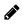
\includegraphics{images/pencil}\textbf{Catatan:}
	
\begin{itemize}
\item Untuk memastikan kelas turunan hanya mempunyai sebuah kelas dasar bersama,
deklarasikan kelas-kelas turunan secara virtual dari kelas dasar. Contoh:

\begin{lstlisting}[language=c++, numbers=none]
class Binatang //<-- common base class (kelas dasar bersama)
class Kuda : virtual public Binatang //<-- penurunan secara virtual
class Burung : virtual public Binatang //<-- penurunan secara virtual
class Kuda_terbang : public Kuda, public Burung
\end{lstlisting}

\item Jika penurunan dilakukan secara virtual seperti di atas, secara otomatis kelas
Kuda\_terbang akan memanggil konstruktor Binatang() walaupun tidak ditulis
secara eksplisit, contoh konstruktor Kuda\_terbang() tanpa memanggil konstruktor
Binatang() berikut ini akan menghasilkan hasil yang sama:
		
\begin{lstlisting}[language=c++, numbers=none]
Kuda_terbang(){//<-- pemanggilan Kuda(), Burung() dan Binatang() implisit
cout << "Konstruktor Kuda_terbang\n";}
\end{lstlisting}
\end{itemize}

\end{quotation}




\section{Masalah Pada Multiple
Inheritance}\label{masalah-pada-multiple-inheritance}

Meskipun multiple inheritance menawarkan banyak keuntungan dibanding
penurunan tunggal, banyak pemrogram C++ menghindari penggunaan multiple
inheritance. Mereka mengatakan bahwa multiple inheritance membuat
pelacakan kesalahan menjadi lebih sulit, dengan mengembangkan kelas
multiple inheritance hirarki semakin rumit dan semakin berisiko
dibandingkan penurunan tunggal dan bahwa hampir semua yang bisa
dilakukan dengan multiple inheritance juga dapat dilakukan dengan single
inheritance. Bahasa pemrograman lain seperti Java dan C\# tidak
mendukung multiple inheritance dengan alasan yang sama. Oleh karena itu,
jika bisa dilakukan dengan cara single inheritance jangan memakai
multiple inheritance.

\begin{quotation}
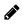
\includegraphics{images/pencil}	\textbf{Catatan}
	\begin{itemize}
		\item Pakailah multiple inheritance jika suatu kelas baru memerlukan
		fitur-fitur yang ada di dua kelas yang berbeda.
		\item Pakailah penurunan secara virtual jika ada lebih dari satu kelas turunan
		namun hanya diperlukan sebuah instan dari kelas dasar.
		\item Pasti terjadi pemanggilan konstruktor kelas dasar bersama (shared base
		class) dari kelas turunan paling bawah (multiple inheritance) ketika
		memakai kelas dasar virtual.
	\end{itemize}
\end{quotation}
 

